\documentclass{cheat-sheet}

\pdfinfo{
  /Title (Zusammenfassung Algebraische Topologie)
  /Author (Tim Baumann)
}

\usepackage{tikz}
\usetikzlibrary{matrix,shapes,arrows,positioning}

\newcommand{\Tau}{\mathcal{T}} % Großes Tau
%\newcommand{\inte}{\mathop{\mathrm{int}}} % Inneres (interior)
%\newcommand{\conv}{\mathop{\mathrm{conv}}} % Konvexe Hülle
%\newcommand{\rel}{\text{ rel }} % = relativ (Homotopie)
%\newcommand{\Ob}{\mathrm{Ob}} % Objects (of a category)
%\newcommand{\Aut}{\mathrm{Aut}} % Automorphisms
%\newcommand{\Mor}{\mathrm{Mor}} % Morphisms
%\newcommand{\dom}{\mathrm{dom}} % Domain
%\newcommand{\codom}{\mathrm{codom}} % Codomain
%\newcommand{\op}{\text{op}} % Duale Kategorie
%\newcommand{\Deck}{\mathrm{Deck}} % Gruppe der Decktransformationen

\newcommand{\angles}[1]{\langle #1 \rangle}
\newcommand{\Simpl}{\mathcal{S}} % Simplizialkomplex
\newcommand{\Real}[1]{\abs{#1}} % geometrische Realisierung
\newcommand{\CC}[1]{{#1}_{\bullet}} % Kettenkomplex (chain complex)
\newcommand{\Top}{\mathbf{Top}} % Kategorie der topologischen Räume
\newcommand{\AbGrp}{\mathbf{AbGrp}} % Kategorie der abelschen Gruppen
\newcommand{\RH}{\tilde{H}} % Reduzierte Homologie
\newcommand{\inte}{\mathop{\mathrm{int}}} % Inneres (interior)
\newcommand{\clos}[1]{\overline{#1}} % Abschluss
\newcommand{\Tor}{\mathrm{Torsion}} % Torsion
\newcommand{\tr}{\mathop{\mathrm{tr}}} % Spur (trace)
\newcommand{\rk}{\mathop{\mathrm{rk}}} % Rang (rank)
\newcommand{\Hom}{\mathop{\mathrm{Hom}}} % Homomorphisms
\newcommand{\cell}{\text{cell}} % zellulär

% Kleinere Klammern
\delimiterfactor=701


\begin{document}

\maketitle{Zusammenfassung Algebr. Topologie}

% Vorlesung vom 8.10.2014

% TODO: Definition $C_n$

%\[ \partial \angles{p_0, ..., p_n} \coloneqq \sum_{i=0}^n (-1)^{i} \angles{p_0, ..., \hat{p_i}, ..., p_n} \]
%\[ \partial_n : C_n \to C_{n-1} \]
%\[ Z_n(S) \coloneqq \ker \partial_n \subset C_n(S) \]
%\[ B_n(S) \coloneqq \im \partial_{n+1} \subset C_n(S) \]


% §2. Simpliziale und singuläre Homologie

\begin{defn}
  Ein \emph{affines $n$-Simplex} ist die konvexe Hülle von $n+1$ affin unabhängigen Punkten $p_0, ..., p_{n+1} \in \R^N$. Die konvexe Hülle von einer Teilmenge dieser Eckpunkte wird \emph{Seite} genannt.\\
  Das \emph{Standard-$n$-Simplex} $\Delta_n$ ist das von den $n+1$ Standard-Basisvektoren im $\R^{n+1}$ aufgespannte Simplex.
\end{defn}

\begin{defn}
  Ein (endlicher) \emph{geometrischer Simplizialkomplex} ist eine (endliche) Menge $\mathcal{S}$ endlich vieler affiner Simplizes im $\R^N$, sodass:
  \begin{itemize}
    \item Ist $K \in \Simpl$ und $T \subset K$ eine Seite von $K$, dann ist auch $T \in \Simpl$.
    \item Für alle $K_1, K_2 \in \Simpl$ ist $K_1 \cap K_2$ entweder eine Seite von $K_1$ und $K_2$ oder leer.
  \end{itemize}
\end{defn}

\begin{defn}
  Jeder Simplizialkomplex $\Simpl$ ist eine \emph{Triangulierung} seines \emph{Polyeders}, dem topologischen Raum $\Real{S} \coloneqq \bigcup_{K \in \Simpl} K$.
\end{defn}

\begin{defn}
  Ein geometrischer Simplizialkomplex mit einer Totalordnung auf der Menge der Eckpunkte heißt \emph{geordnet}.
\end{defn}

\begin{nota}
  Ein $n$-Simplex mit Eckpunkten $v_0, ..., v_n$ in einem geordneten geom. Simplizialkomplex wird mit $\angles{v_0, ..., v_n}$ bezeichnet, falls $v_0 < v_1 < ... < v_n$.
\end{nota}

\begin{nota}
  $\Simpl_n \coloneqq \Set{\sigma \in \Simpl}{\text{$\sigma$ ist geordneter $n$-Simplex}}$
\end{nota}

\begin{defn}
  Eine \emph{simpliziale $n$-Kette} in einem geordneten geom. Simplizialkomplex ist eine endliche formale Linearkombination
  \[ \sum_{\sigma \in \Simpl_n} \lambda_\sigma \cdot \sigma, \]
  wobei $\lambda_\sigma \in \Z$. Die Menge solcher Linearkombinationen ist $C_n(\Simpl)$.\\
  Sie ist die freie abelsche Gruppen über der Menge der Simplizes.
\end{defn}

\begin{bem}
  $C_n(\Simpl)$ ist eine Gruppe.
\end{bem}

\begin{defn}
  Der Rand eines orientierten $n$-Simplex $\angles{v_0, ..., v_n} \in \Simpl$ ist
  \[ \delta \angles{v_0, ..., v_n} \coloneqq \sum_{i=0}^n (-1)^i \angles{v_0, ..., \hat{v_i}, ..., v_n}. \]
  Durch lineare Fortsetzung erhalten wir einen Gruppenhomo $\partial_n : C_n(\Simpl) \to C_{n-1}(\Simpl)$.
\end{defn}

% Vorlesung vom 8.10.2014

\begin{defn}
  Ein \emph{Kettenkomplex} $\CC{C}$ ist eine Folge $(C_n)_{n \in \N}$ von abelschen Gruppen und Gruppenhomomorphismen $\partial_n : C_n \to C_{n-1}$ mit der Eigenschaft $\partial_{n-1} \circ \partial_n = 0$.
\end{defn}

\begin{defn}
  Sei $\CC{C}$ ein Kettenkomplex.
  \begin{itemize}
    \item $Z_n(\CC{C}) \coloneqq \ker \partial_n \subset C_n(\CC{C})$ heißt Gruppe der \emph{$n$-Zykel},
    \item $B_n(\CC{C}) \coloneqq \im \partial_{n+1} \subset Z_n(\CC{C})$ heißt Gruppe der \emph{$n$-Ränder},
    \item $H_n(\CC{C}) \coloneqq Z_n(\CC{C}) / B_n(\CC{C})$ heißt \emph{$n$-te Homologiegruppe}.
  \end{itemize}
\end{defn}

% 2.1
\begin{prop}
  Für $n \geq 1$ gilt $\partial_{n-1} \circ \partial_n = 0$. Die simplizialen $n$-Ketten bilden also einen Kettenkomplex.
\end{prop}

\begin{defn}
  Ein \emph{singuläres $n$-Simplex} in einem topologischen Raum $X$ ist eine stetige Abbildung $\sigma : \Delta^n \to X$. Wir bezeichnen mit $\Delta_n(X)$ die Menge der singulären $n$-Simplizes in $X$ und mit $C_n(X)$ die freie abelsche Gruppe über $\Delta_n(X)$. Wir definieren
  \[
    \partial_n : C_n(X) \to C_{n-1}(X), \quad
    \sigma \mapsto \sum_{i=0}^n (-1)^i \sigma_{\angles{e_o,...,\hat{e_i},...,e_n}}.
  \]
  Analog zu oben gilt $\partial_{n-1} \circ \partial_n = 0$, man erhält also einen Komplex $\CC{C}(X)$ der singulären Ketten in $X$. Dessen Homologiegruppen heißen \emph{singuläre Homologiegruppen} $H_n(X)$.
\end{defn}

\begin{defn}
  Eine \emph{Kettenabbildung} zwischen Kettenkomplexen $\CC{C}$ und $\CC{D}$ ist eine Familie $(f_n : C_n \to D_n)_{n \in \N}$ von Gruppenhomomor- phismen, welche mit dem Differential verträglich sind, d.\,h.
  \[ \fa{n \in \N} \partial_n^{(D)} \circ f_n = f_{n-1} \circ \partial_n^{(C)}. \]
  Aus einer solchen Abbildung erhält man wiederum eine Abbildung $H_n(f) : H_n(\CC{C}) \to H_n(\CC{C})$ für alle $n \in \N$. Somit definiert $H_n$ einen Funktor von der Kategorie der Kettenkomplexe in die Kategorie der abelschen Gruppen.
\end{defn}

% Ausgelassen: Kettenisomorphismus

\begin{defn}
  Für eine Abbildung $f : X \to Y$ von topologischen Räumen erhalten wir eine Abbildung $f_* : \CC{C}(X) \to \CC{C}(Y)$ definiert durch $f_*(\sigma) \coloneqq f \circ \sigma$ für ein $n$-Simplex $\sigma : \Delta_n \to X$. Die Zuordnung $f \mapsto f_*$ erfüllt die Funktiorialitätsaxiome. Somit definiert $H_n$ für alle $n \in \N$ einen Funktor $\Top \to \AbGrp$.
\end{defn}

\begin{kor}
  Homöomorphe Räume haben isomorphe singuläre Homologiegruppen.
\end{kor}

% Vorlesung vom 23.10.2014

\begin{prop}
  Sei $\pi_0(X)$ die Menge der Wegekomponenten von $X$. Die Inklusionen $A \hookrightarrow X$ (für $A \in \pi_0(X)$) induzieren einen Isomorphismus
  \[ \bigoplus_{A \in \pi_0(X)} H_*(A) \cong H_*(X). \]
\end{prop}

\begin{prop}
  Sei $X \not= \emptyset$ wegzusammenhängend. Dann ist $H_0(X) \cong \Z$.
\end{prop}

\begin{defn}
  Eine \emph{Kettenhomotopie} zw. Kettenabb. $\phi_*, \psi_* : \CC{C} \to \CC{D}$ ist eine Folge von Homomorphismen $P_n : C_n \to D_{n+1}$ mit
  \[ \fa{n \in \N} \partial_{n+1} \circ P_n + P_{n-1} \circ \partial_n = \phi_n - \psi_n. \]
\end{defn}

\begin{prop}
  Seien $\phi_*, \psi_* : \CC{C} \to \CC{D}$ kettenhomotop. Dann gilt
  \[ H_*(\phi_*) = H_*(\psi_*) : H(\CC{C}) \to H(\CC{D}). \]
\end{prop}

\begin{satz}
  Seien $f, g : X \to Y$ homotope Abbildungen. Dann sind $f_*, g_* : \CC{X} \to \CC{Y}$ kettenhomotop.
\end{satz}

\begin{kor}
  \begin{itemize}
    \item Seien $f, g : X \to Y$ homotope Abbildungen. Dann gilt
    \[ f_* = g_* : H_*(X) \to H_*(Y). \]
    \item Homotopieäquivalente Räume haben isomorphe Homologiegruppen.
  \end{itemize}
\end{kor}

% Vorlesung vom 15.10.2014

% §3. Relative Homologie und Ausschneidung

\begin{defn}
  Ein \emph{Unterkomplex} $\CC{D}$ von $\CC{C}$ ist eine Folge von Untergruppen $D_n \subset C_n$, sodass gilt: $\partial D_n \subset D_{n-1}$ für alle $n \geq 1$.
\end{defn}

\begin{defn}
  Ist $\CC{D} \subset \CC{C}$ ein Unterkomplex, so ist der \emph{Quotientenkomplex} $\CC{C}/\CC{D}$ definiert durch
  \[
    (\CC{C}/\CC{D})_n \coloneqq C_n/D_n, \quad
    \partial^{C/D}_n[c] \coloneqq [\partial^C_n(c)].
  \]
\end{defn}

\begin{defn}
  Sei $(X, A)$ ein Raumpaar. Der \emph{relative singuläre Ketten- komplex} $\CC{C}(X, A)$ ist definiert als Quotientenkomplex $\CC{X}/\CC{A}$.\\
  Dessen Homologiegruppen heißen \emph{relative singuläre Homologiegruppen} $H_n(X, A)$.
\end{defn}

\begin{bem}
  $H_n$ ist ein Funktor $\Top(2) \to \AbGrp$.
\end{bem}

\begin{defn}
  Eine Homotopie zwischen Abbildungen von Raumpaaren $f, g : (X, A) \to (Y, B)$ ist eine Homotopie $H : \cinterval{0}{1} \times X \to Y$ zwischen $f$ und $g$ mit $H(\cinterval{0}{1} \times A) \subset Y$.
\end{defn}

\begin{prop}
  Homotope Abbildungen von Raumpaaren induzieren dieselbe Abbildung in relativer Homologie.
\end{prop}

\begin{defn}
  Ein Kettenkomplex heißt \emph{exakt} (oder \emph{azyklisch}), falls seine Homologiegruppen alle Null sind, d.\,h. $\fa{n \in \N} \im \partial_{n+1} = \ker \partial_n$.
\end{defn}

\begin{defn}
  Eine \emph{kurze exakte Sequenz} (keS) ist ein exakter Kettenkomplex der Gestalt
  \[ 0 \to A \to B \to C \to 0. \]
\end{defn}

\begin{defn}
  Eine \emph{kurze exakte Sequenz von Kettenkomplexen} ist ein Diagramm der Form
  \[ 0 \to \CC{A} \to \CC{B} \to \CC{C} \to 0, \]
  in jedem Grad eine kurze exakte Sequenz
  \[ 0 \to A_n \to B_n \to C_n \to 0. \]
\end{defn}

\begin{bem}
  Ist $(X, A)$ ein Raumpaar, so erhält man eine kurze exakte Sequenz
  \[ 0 \to \CC{C}(A) \to \CC{C}(X) \to \CC{C}(X, A) \to 0. \]
  Für ein Raumtripel $(X, A, U)$ erhält man eine k.\,e.\,S.
  \[ 0 \to \CC{C}(A, U) \to \CC{C}(X, U) \to \CC{C}(X, A) \to 0. \]
\end{bem}

% 3.2
\begin{prop}[Schlangenlemma]
  Die ex. Sequenz $0 \to \CC{A} \to \CC{B} \to \CC{C} \to 0$ induziert in jedem Grad einen sogenannten \emph{verbindenden Homomorphismus} $\partial_n : H_n(C) \to H_{n-1}(A)$, sodass die Sequenz
  \[ ... \to H_n(A) \to H_n(B) \to H_n(C) \xrightarrow{\partial_n} H_{n-1}(A) \to H_{n-1}(B) \to ... \]
  exakt ist. Diese Sequenz wird \emph{lange exakte Sequenz} genannt.
\end{prop}

\begin{kor}
  Sei $(X, A)$ ein Raumpaar. Dann gibt es Homomorphis- men $\partial_n : H_n(X, A) \to H_{n-1}(A)$, sodass die Sequenz
  \[
    ... \to H_n(A) \to H_n(X) \to H_n(X, A) \xrightarrow{\partial_n} H_{n-1}(A) \to ...
    \quad \text{exakt ist.}
  \]
  Für ein Raumtripel $(X, A, U)$ erhält man eine l.\,e.\,S.
  \[
    ... \to H_n(A, U) \to H_n(X, U) \to H_n(X, A) \xrightarrow{\partial_n} H_{n-1}(A, U) \to ...
  \]
\end{kor}

\begin{defn}
  Die \emph{reduzierte Homologie} $\RH_*(X)$ eines topologischen Raumes $X$ ist die Homologie des Kettenkomplexes
  \[ ... \to C_2(X) \xrightarrow{\partial_n} C_1(X) \xrightarrow{\partial_1} C_0(X) \xrightarrow{\epsilon} \to \Z \to 0, \]
  wobei $\epsilon$ der sogenannte \emph{Augmentierungshomomorphismus} ist:
  \[ \epsilon : \sum_{\sigma \in \Delta_0(X)} \lambda_\sigma \cdot \sigma \mapsto \sum_{\sigma} \lambda_\sigma \in \Z. \]
\end{defn}

\begin{prop}
  \begin{itemize}
    \item $\RH_n(X) = H_n(X)$ für $n \geq 1$
    \item Ist $X = \emptyset$, so ist $\RH_n(X) = 0$ für $n \geq 0$ und $\RH_{-1}(X) = \Z$.
    \item Ist $X \not= \emptyset$, so ist $H_n(X) \cong \RH_n(X) \oplus \Z$, jedoch nicht kanonisch.
    \item Ist $X$ kontrahierbar, so gilt $\RH_n(X) = 0$ für alle $n \in \N$.
    \item Ist $(X, A)$ ein Raumpaar, so gibt es eine lange exakte Sequenz
    \[ ... \to \RH_0(A) \to \RH_0(X) \to \RH_0(X,A) \to \RH_{-1}(A) \to \RH_{-1}(X) \to 0 \]
  \end{itemize}
\end{prop}

% Vorlesung vom 20.10.2014

% 3.5
\begin{satz}
  Sei $(X, A)$ ein Raumpaar, $U \subset A$ mit $\clos{U} \subset \inte A$. Dann induziert die Inklusion $(X - U, A - U) \hookrightarrow (X, A)$ Isomorphismen
  \[ H_n(X - U, A - U) \to H_n(X, A) \quad \text{für alle $n \geq 0$.} \]
\end{satz}

\begin{bem}
  Eine äquivalente Aussage zum Ausschneidungssatz ist:\\
  Seien $A, B \subset X$ mit $X = \inte A \cup \inte B$. Dann induziert die Inklusion $(B, A \cap B) \to (X, A)$ Isomorphismen in Homologie.
\end{bem}

% Vorlesung vom 22.10.2014

% Ausgelassen: Hilfspropositionen zum Beweis des Ausschneidungssatzes, U-feine Ketten etc.

% Vorlesung vom 27.10.2014

\begin{defn}[\emph{Eilenberg-Steenrod-Axiome}]
  Eine \emph{Homologietheorie} ist eine Folge von Funktoren
  \[ H_n : \Top(2) \to \AbGrp, \]
  und natürlichen Transformationen
  \[ \delta_n : H_n(X, A) \to H_{n-1}(A, \emptyset) \]
  mit den folgenden Eigenschaften:
  \begin{itemize}
    \item \emph{Homotopieinvarianz}: Seien $f, g : (X, A) \to (B, Y)$ homotop als Abbildungen von Raumpaaren. Dann gilt $f_* = g_* : H_n(X, A) \to H_n(Y, B)$.
    \item \emph{Lange exakte Sequenz}: Die Inklusionen $A \hookrightarrow X$ und $(X, \emptyset) \hookrightarrow (X, A)$ induzieren eine l.e.S.
    \[ ... \to H_n(A) \to H_n(X) \to H_n(X, A) \xrightarrow{\partial_n} H_{n-1}(A) \to ... \]
    \item \emph{Ausschneidung}: Ist $U \subset A$ mit $\clos{A} \subset \inte(A)$, dann induziert die Inklusion $(X - U, A - U) \hookrightarrow (X, A)$ Isomorphismen
    \[ H_n(X-U, A-U) \to H_n(X,A). \]
  \end{itemize}
\end{defn}

\begin{defn}
  Die \emph{Koeffizienten} einer Homologietheorie sind die Homologiegruppen $H_n(pt)$ des einpunktigen Raums.
  Eine Homologietheorie heißt \emph{gewöhnlich}, falls $H_n(pt) = 0$ für $n > 0$.
\end{defn}

\begin{bem}
  Manchmal fordert man auch das Summenaxiom: Für eine Familie $(X_i)_{i \in I}$ von topologischen Räumen induzieren die Inklusionen $X_i \hookrightarrow X$ in die disjunkte Summe $X$ aller $X_i$ einen Iso
  \[ \bigoplus_{i \in I} H_n(X_i) \xrightarrow{\cong} H_n(X). \]
\end{bem}

\begin{bem}
  Die singuläre Homologie ist eine gewöhnliche Homologietheorie, die das Summenaxiom erfüllt.
\end{bem}

% §4. Erste Berechnungen und Anwendungen

\begin{defn}
  Ein Raumpaar $(X, A)$ heißt \emph{gut}, falls $A$ nicht leer, abgeschlossen und starker Deformationsretrakt einer offenen Umgebung ist.
\end{defn}

\begin{prop}
  Sei $(X, A)$ ein gutes Raumpaar. Dann induziert $q : (X, A) \to (X/A, A/A)$ Isomorphismen
  \[ H_n(X, A) \to H_n(X/A, A/A) = \RH_n(X/A) \quad \text{für alle $n \in \N$.} \]
\end{prop}

% 4.3
\begin{satz}
  Für $n \geq 0$ ist $S^n$ kein Retrakt von $D^{n+1}$.
\end{satz}

% 4.4
\begin{kor}[\emph{Brouwerscher Fixpunktsatz}]\mbox{}\\
  Jede stetige Abbildung $f : D^n \to D^n$ hat einen Fixpunkt.
\end{kor}

% 4.5
\begin{satz}[Topologische Invarianz der Dimension]\mbox{}\\
  Seien $U \opn R^n$ und $V \opn \R^m$ homöomorph. Dann gilt $n = m$.
\end{satz}

% Vorlesung vom 29.10.2014

\begin{defn}
  Sei $f : S^n \to S^n$ stetig. In Homologie induziert $f$ eine Abbildung $H_n(f) : \Z \to \Z$, die durch Multiplikation mit einer ganzen Zahl gegeben ist. Diese Zahl heißt \emph{Abbildungsgrad} $\deg f$ von $f$.
\end{defn}

\begin{lem}
  \begin{itemize}
    \item $\deg (f \circ g) = (\deg f) \cdot (\deg g)$.
    \item $H_n(f)$ ist genau dann ein Isomorphismus, wenn $\deg(f) = \pm 1$.
  \end{itemize}
\end{lem}

\begin{prop}
  Sei $f : S^n \to S^n$ die Spiegelung an einer Hyperebene $H \subset \R^{n+1}$. Dann gilt $\deg f = -1$.
\end{prop}

\begin{defn}
  Ein \emph{Vektorfeld} über $S^n$ ist eine stetige Abbildung $v : S^n \to \R^{n+1}$, sodass $v(x) \perp x$ für alle $x \in S^n$.
\end{defn}

% 4.7
\begin{satz}
  Die Sphäre $S^n$, $n \geq 1$ hat genau dann ein nirgends verschwindendes Vektorfeld, wenn $n$ ungerade ist.
\end{satz}

% 4.8
\begin{satz}
  Sei $n$ gerade und wirke eine Gruppe $G$ frei auf $S^n$. Dann ist entweder $G = \{ e \}$ oder $G \cong \Z_2$.
\end{satz}

% Vorlesung vom 3.11.2014

\begin{defn}
  Sei $f : S^n \to S^n$ stetig, $x \in S^n$, sodass eine Umgebung $U$ von $x$ existiert mit $U \cap f^{-1}(f(x)) = \{ x \}$. Mit Ausschneidung und der l.e.S. erhält man Isomorphismen
  \[ H_k(U, U - \{ x \}) \cong H_k(S^n, S^n - \{ x \}) \cong \RH_k(S^n) \cong \Z. \]
  Die induzierte Abb. $f_* : H_n(U, U - \{ x \}) \to H_n(S^n, S^n - \{ f(x) \})$ ist gegeben durch Multiplikation mit einer ganzen Zahl. Diese heißt \emph{lokaler Abbildungsgrad} ($\deg f|x$) von $f$ bei $x$.
  %(und hängt nicht von $U$ ab).
\end{defn}

% 4.9
\begin{prop}
  Sei $f : S^n \to S^n$ stetig und $y {\in} S^n$ mit $f^{-1}(y) = \{ x_1, ..., x_n \}$.\\
  Dann ist $\deg f|x_i$ definiert für $i = 1, ..., n$ und es gilt
  \[ \deg f = \sum_{i=1}^n \deg f|x_i. \]
\end{prop}

\begin{prop}
  Sei $f : S^n \to S^n$ stetig. Dann gilt
  \[ \deg f = \deg (\Sigma f : \Sigma S^n \to \Sigma S^n). \]
\end{prop}

% 4.11
\begin{prop}
  Seien $A, B \subset X$ mit $X = A \cup B$. Angenommen, es gibt Umgebungen $U$ von $A$ und $V$ von $B$, sodass die Inklusionen $A \hookrightarrow U$, $B \hookrightarrow V$ und $A \cap B \hookrightarrow U \cap V$ Homotopieäquivalenzen sind. Dann existiert die \emph{Mayer-Vietoris-Sequenz}
  \[ ... \to H_*(A \cap B) \to H_*(A) \oplus H_*(B) \to H_*(X, A \cap B) \to H_{*-1}(A \cap B) \to ... \]
\end{prop}

% 4.12
\begin{prop}[Verallg. Jordanscher Kurvensatz]
  % Weggelassen: Teil 1
  Sei $S \subset S^n$ ein Teilraum, der zu einer Sphäre $S^k \subset \R^{k+1}$ homöomorph ist. Dann ist $k \leq n$ und
  \[ \RH_i(S^n - S) = \begin{cases}
    \Z, & \text{falls $i = n - k - 1$,} \\
    0, & \text{sonst.}
  \end{cases} \]
\end{prop}

\begin{kor}[Jordanscher Kurvensatz]
  Sei $\phi : S^1 \to \R^2$ eine stetige Einbettung. Dann besteht $\R^2 - \phi(S^1)$ aus zwei Komponenten, von denen genau eine beschränkt ist.
\end{kor}

% Ausgelassen: Lemma 4.14 und 4.15 über (Wege-)komponenten
% Ausgelassen: Proposition 4.16 (Verschärfung des Jordanschen Kurvensatzes)

% 4.17
\begin{satz}[Invarianz des Gebietes]
  Sei $U \subset \R^n$ offen und $\phi : U \to \R^n$ stetig und ein Homöomorphismus auf das Bild. Dann ist $\phi(U)$ offen. %in $\R^n$
\end{satz}

% Vorlesung vom 12.11.2014

% §5. $\Delta$-Komplexe, CW-Komplexe und ihre Homologie

\begin{defn}
  Ein $\Delta$-Komplex ist ein topologischer Raum $X$ zusammen mit einer Familie $(\sigma_\alpha : \Delta^{n(\alpha)} \to X)_{\alpha \in I}$ von stetigen Abbildungen (genannt \emph{charakteristische Abbildungen}), sodass:
  \begin{itemize}
    \item Die Restriktionen $\sigma_\alpha|\inte(\Delta^{n(\alpha)}) : \inte(\Delta^{n(\alpha)}) \to X$ sind injektiv und jeder Punkt $x \in X$ liegt im Bild (genannt \emph{offenes Simplex}) von genau einer solchen Restriktion.
    \item Ist $\sigma_\alpha : \Delta^{n(\alpha)} \to X$ eine char. Abb. und $\tau \subset \Delta^{n(\alpha)}$ eine ($n(\alpha)-1$)-dimensionale Seite, dann ist $\sigma_\alpha|\tau : \Delta^{n(\alpha)-1} \to X$ wieder eine charakteristische Abbildung.
    \item $A \subset X$ ist offen $\iff$ alle $\sigma_\alpha^{-1}(A)$ sind offen in $\Delta^{n(\alpha)}$.
  \end{itemize}
\end{defn}

\begin{bem}
  Jeder endliche geordnete Simplizialkomplex trägt die Struktur eines $\Delta$-Komplexes.
\end{bem}

\begin{bem}
  Alternativ ist ein $\Delta$-Komplex ein kontravarianter Funktor von der Kategorie $\Delta$ der endlichen total geordneten Mengen mit streng monotonen Abbildungen in die Kategorie der Mengen.
\end{bem}

\begin{defn}
  Für einen $\Delta$-Komplex $X$ sei $C_n^\Delta(X)$, die freie abelsche Gruppe erzeugt von den Abbildungen $\sigma_\alpha : \Delta^{n(\alpha)} \to X$ mit $n(\alpha) = n$. Diese Gruppen bilden einen Simplizialkomplex. Die Homologiegruppen dieses Komplexes heißen \emph{simpliziale Homologiegruppen} $H^\Delta_*(X)$.
\end{defn}

\begin{defn}
  Ein \emph{Teilkomplex} eines $\Delta$-Komplexes ist eine Teilmenge der charakteristischen Abbildungen (zusammen mit der Vereinigung der Bilder dieser Abbildungen als topologischer Raum), die selbst die Axiome für einen Delta-Komplex erfüllt.
\end{defn}

\begin{defn}
  Das \emph{$k$-Skelett} eine $\Delta$-Komplexes ist der Teilkomplex, der aus den Bildern aller $i$-Simplizes besteht, wobei $i \leq k$.
\end{defn}

\begin{defn}
  Die \emph{relative singuläre Homologie} $H_n^\Delta(X, A)$ des $\Delta$-Komplexes $X$ bzgl. eines Teilkomplexes $A$ ist die Homologie des Quotientenkomplexes $C_n^\Delta(X)/C_n^\Delta(A)$.
\end{defn}

% 5.1
\begin{satz}
  Sei $X$ ein $\Delta$-Komplex und $A \subset X$ ein Unterkomplex. Dann induziert die Inklusion $C_*^\Delta(X) \hookrightarrow C_*(X)$ Isomorphismen von Homologiegruppen.
\end{satz}

% 5.2
\begin{lem}
  Für $n \geq 0$ gilt
  \[
    H^\Delta_i(\Delta^n, \partial \Delta^n) \cong
    H_i(\Delta^n, \partial \Delta^n) =
    \begin{cases}
      \Z, & \text{für $i=n$} \\
      0, & \text{sonst}
    \end{cases}
  \]
  und die Homologieklasse von $\id : \Delta^n \to \Delta^n$ erzeugt sowohl $H^\Delta_n(\Delta^n, \partial \Delta^n)$ als auch $H_n(\Delta^n, \partial \Delta^n)$
\end{lem}

\begin{lem}[\emph{Fünferlemma}]
  Sei folgendes kommutatives Diagramm von $R$-Modulen mit exakten Zeilen gegeben:
  \begin{center}
    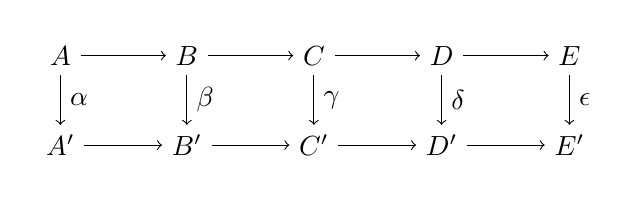
\begin{tikzpicture}
      \matrix (mat) [matrix of nodes, column sep=1cm, row sep=0.65cm]{
        \node (A) {$A$}; &
        \node (B) {$B$}; &
        \node (C) {$C$}; &
        \node (D) {$D$}; &
        \node (E) {$E$}; \\
        \node (A') {$A'$}; &
        \node (B') {$B'$}; &
        \node (C') {$C'$}; &
        \node (D') {$D'$}; &
        \node (E') {$E'$}; \\
      };
      \draw[->] (A) to node {} (B);
      \draw[->] (B) to node {} (C);
      \draw[->] (C) to node {} (D);
      \draw[->] (D) to node {} (E);
      \draw[->] (A') to node {} (B');
      \draw[->] (B') to node {} (C');
      \draw[->] (C') to node {} (D');
      \draw[->] (D') to node {} (E');
      \draw[->] (A) to node [right] {$\alpha$} (A');
      \draw[->] (B) to node [right] {$\beta$} (B');
      \draw[->] (C) to node [right] {$\gamma$} (C');
      \draw[->] (D) to node [right] {$\delta$} (D');
      \draw[->] (E) to node [right] {$\epsilon$} (E');
    \end{tikzpicture}
  \end{center}
  Angenommen, $\alpha$, $\beta$, $\delta$ und $\epsilon$ sind Isomorphismen. Dann ist auch $\gamma$ ein Isomorphismus.
\end{lem}

% Vorlesung vom 17.11.2014

\begin{defn}
  Ein \emph{CW-Komplex} ist ein topologischer Raum $X$ mit einer Folge von abgeschlossenen Unterräumen
  \[
    X^0 \subset X^1 \subset X^2 \subset ... \subset X, \quad
    \bigcup_{i \geq 0} X^i = X,
  \]
  genannt \emph{$i$-Skelette} $X^i$, sodass gilt:
  \begin{itemize}
    \item $X^0$ ist eine diskrete Menge von Punkten.
    \item Für alle $n \geq 1$ gibt es eine Familie von \emph{Anheftungsabb'en} $(\phi_\alpha : \partial D^n_\alpha \to X^{n-1})_{\alpha \in I(n)}$ (dabei ist $D^n_\alpha$ eine Kopie von $D^n$), sodass
    \[ X^n = X^{n-1} \cup_{(\phi_\alpha)_{\alpha \in I(n)}} \coprod_{\alpha \in I(n)} D^n_\alpha. \]
    \item $X$ trägt die Finaltopologie bzgl. obiger Filtrierung, d.\,h. \\
    $A \subset X$ ist abgeschlossen $\iff$ alle $A \cap X^i$ sind abgeschlossen.
  \end{itemize}
\end{defn}

\begin{defn}
  Ein CW-Komplex heißt \emph{endlich-dimensional}, falls $X^i = X$ für ein $i \in \N$. Er heißt \emph{endlich}, falls er insgesamt nur endlich viele Anheftungsabb'en besitzt (dann ist er insbesondere endlich-dim).
\end{defn}

\begin{prop}
  CW-Komplexe sind normal (und damit Hausdorffsch).
\end{prop}

\begin{defn}
  Die Anheftungsabb'en $\phi_\alpha : \partial D^{n}_\alpha \to X^{n-1}$ lassen sich kanonisch fortsetzen zu \emph{charakteristischen Abb'en} $\Phi_\alpha : D^n_\alpha \to X^n \subset X$.\\
  Die Bilder dieser Abb'en werden \emph{abgeschlossene Zellen} genannt.\\
  Die Bilder der Einschränkungen $\Phi_\alpha|\inte(D^n_\alpha)$ heißen \emph{Zellen} von $X$ und werden mit $e^n_\alpha$ bezeichnet.
\end{defn}

\begin{prop}
  \begin{itemize}
    \item $\Phi_\alpha|\inte(D^n_\alpha) : \inte(D^n_\alpha) \to X^n$  ist eine topologische Einbettung (d.\,h. ein Homöo auf das Bild).
    \item Jeder Punkt aus $X$ liegt in genau einer Zelle.
    \item Der Abschluss einer Zelle ist eine abgeschlossene Zelle.
    \item Jede abgeschlossene Zelle trifft nur endlich viele Zellen.
  \end{itemize}
\end{prop}

% Vorlesung vom 19.11.2014

\begin{defn}
  Ein \emph{Unterkomplex} eines CW-Komplexes ist eine Teilmenge $A \subset X$, die selbst ein CW-Komplex ist, und zwar so, dass alle anheftenden Abb'en von $A$ auch anheftende Abb'en von $X$ sind.
\end{defn}

\begin{defn}
  Ein \emph{CW-Paar} ist ein Raumpaar $(X, A)$, wobei $X$ ein CW-Komplex und $A$ ein Unterkomplex von $X$ ist.
\end{defn}

% 5.6
\begin{prop}
  \begin{itemize}
    \item $X^n$ ist ein Unterkomplex von $X$ und von $X^m$ für $m \geq n$.
    \item CW-Raumpaare sind gute Raumpaare.
    \item Jede Zelle eines CW-Komplexes ist in einem endlichen Unterkomplex enthalten.
  \end{itemize}
\end{prop}

\begin{defn}
  Die \emph{Einpunktvereinigung} einer Familie $(X_i, x_i)_{i \in I}$ von punktierten Räumen ist
  \[ \bigvee_{i \in I} X_i \coloneqq \left( \bigsqcup_{i \in I} X_i \right) / \Set{x_i}{i \in I}. \]
  Man erhält Projektionen $q_j : \vee_i X_i \to X_j$ durch Abbilden aller Punkte aus $X_i$, $i \not= j$. auf den Basispunkt $x_j$.
\end{defn}

% 5.7
\begin{prop}
  Sei $(X_i, x_i)_{i \in I}$ eine Familie von punktierten Räumen, sodass alle Raumpaare $(X_i, \{ x_i \})$ gut sind. Dann induzieren die Inklusionen $X_i \hookrightarrow \vee_i X_i$ einen Isomorphismus
  \[
    \bigoplus_{i \in I} \RH_n(X_i) \cong \RH_n\left( \vee_i X_i \right) \quad
    \text{für alle $n \geq 0$.}
  \]
\end{prop}

% 5.8
\begin{lem}
  Sei $X$ ein CW-Komplex. Dann gilt
  \[ X^n/X^{n-1} \approx \vee_{i \in I(n)} S^n. \]
\end{lem}

\begin{kor}
  $H_i(X^n/X^{n-1}) = \begin{cases}
    \oplus_{i \in I(n)} \Z, & \text{falls } i = n, \\
    0, & \text{sonst.}
  \end{cases}$
\end{kor}

% 5.9
\begin{prop}
  \begin{itemize}
    \item $H^k(X^n) = 0$ für $k > n$.
    \item Für $k < n$ induziert die Inklusion $X^n \hookrightarrow X$ Isomorphismen $H_k(X^n) \cong H_k(X)$.
  \end{itemize}
\end{prop}

\begin{defn}
  Der \emph{zelluläre Kettenkomplex} eines CW-Komplexes $X$ ist definiert durch
  \[ C^\cell_n(X) \coloneqq H_n(X^n, X^{n-1}) \]
  mit dem verbindenden Homomorphismus
  \[ \partial_n : H_n(X^n, X^{n-1}) \to H_{n-1}(X^{n-1}, X^{n-2}) \]
  aus der l.\,e.\,S. des Raumtripels $(X^n, X^{n-1}, X^{n-2})$ als Randabb.\\
  Dabei setzt man $X^{n-2} \coloneqq \emptyset$ und $\partial_0 = 0$.\\
  Die Homologiegruppen dieses Komplexes werden mit $H_*^\cell(X)$ bezeichnet.
\end{defn}

\begin{prop}
  % Ausgelassen: Erster Teil
  Für jeden CW-Komplex $X$ gilt $H_*^\cell(X) \cong H_*(X)$.
\end{prop}

\begin{kor}
  Hat der CW-Komplex $X$ keine $n$-Zellen so ist $H_n(X) = 0$. Wenn $X$ $k$-viele $n$-Zellen besitzt, dann wird $H_n(X)$ von höchstens $k$ Elementen erzeugt.
\end{kor}

\begin{bem}
  Wir wählen Erzeuger $t_n$ von $H_n(D^n, \partial D^n)$ und $s_n$ von $\RH_n(S^n)$ wie folgt:
  Für $n=0$ wählen wir einen beliebigen Erzeuger von $H_0(S^0)$. Angenommen, wir haben einen Erzeuger von $s_i \in H_i(S^i)$ bereits definiert. Der verbindende Homomorphismus $\partial_i : H_{i+1}(D^{i+1}, S^i) \to H_i(S^i)$ aus der l.\,e.\,S. des Raumpaares $(D^{i+1}, S^i)$ ist ein Isomorphismus. Sei der Erzeuger $t_{i+1}$ von $H_{i+1}(S^{i+1})$ das Urbild von $s_i$ unter $\partial_i$. Wir wählen $s_{i+1}$ als das Bild von $t_{i+1}$ unter dem Isomorphismus
  \[ H_{i+1}(D^{i+1}, S^i) \cong H_{i+1}(D^{i+1}/S^i) \cong H_{i+1}(S^{i+1}) \]
  Dabei seien die Homöomorphismen $D^{i+1}/S^i \approx S^{i+1}$ fest gewählt.\\
  Wir erhalten Isomorphismen
  \[ C^{\cell}_n(X) = H_n(X^n, X^{n-1}) \cong \bigoplus_{I(n)} H_n(D^n, S^{n-1}) \cong \bigoplus_{I(n)} \Z. \]
  Sei nun $e^n_\alpha$ eine $n$-Zelle mit anheftender Abb. $\phi_\alpha : S^{n-1} \to X^{n-1}$ und $e^{n-1}_\beta$ eine $(n{-}1)$-Zelle von $X$. Sei $d_{\alpha \beta}$ der Abbildungsgrad von
  \[ S^{n-1} \xrightarrow{\phi_\alpha} X^{n-1} \to X^{n-1} / X^{n-2} \cong \vee_{i \in I(n)} S^{n-1} \xrightarrow{q_\beta} S^{n-1}. \]
  Wir bezeichnen den $\alpha$-ten Erzeuger von $C^{\cell}_n(X)$ (mit $\alpha \in I(n)$) mit $e^n_\alpha$. Dann haben wir:
\end{bem}

\begin{prop}
  Der zelluläre Randoperator ist gegeben durch
  \[ \partial_n(e^n_\alpha) = \!\!\! \sum_{\beta \in I(n-1)} \!\!\! d_{\alpha \beta} e^{n-1}_\beta. \]
  Die Summe ist dabei endlich.
\end{prop}

% Vorlesung vom 26.11.2014

% §6. Homologie mit Koeffizienten, der Satz von Borsuk-Ulam


\begin{defn}
  Der singuläre Kettenkomplex mit Koeffizienten in einer abelschen Gruppe $G$ eines topologischen Raumes $X$ ist def. durch
  \[ C_n(X) \coloneqq \{ \text{ formale endl. Linearkomb. } \sum_{\sigma \in \Delta_n} \lambda_\sigma \cdot \sigma \text{ mit $\lambda_\sigma \in G$} \} \]
  Die Randabbildung ist ganz wie beim gewöhnlichen Kettenkomplex ($G = \Z$) definiert. Die Homologie dieses Komplexes heißt \emph{singuläre Homologie mit Koeffizienten in $G$}. Sie ist eine gewöhnliche Homologietheorie im Sinne von Eilenberg und Steenrod. Man erhält \emph{reduzierte Homologie mit Koeffizienten in $G$}, indem man die Komplex von dem mit dem Augmentierungshomomorphismus
  \[ \epsilon : C_0(X; G) \to G, \quad \sum_{\sigma \in \Delta_0(X)} \lambda_\sigma \cdot \sigma \mapsto \!\!\! \sum_{\sigma \in \Delta_0(X)} \lambda_\sigma \]
  erweiterten Kettenkomplex mit Koeffizienten in $G$ nimmt.
\end{defn}

% 6.1
\begin{prop}
  Ist $f : S^n \to S^n$ stetig vom Grad $n$, so ist %die induzierte Abbildung
  \[ f_* : \RH_n(S^n; G) \to \RH_n(S^n; G) \]
  durch Multiplikation mit $n$ gegeben.
\end{prop}

\begin{defn}
  Ist $X$ ein CW-Komplex, so ist der zelluläre Kettenkomplex mit Koeffizienten in $G$ definiert durch
  \[ C_n^\cell(X) \coloneqq H_n(X^n, X^{n-1}; G). \]
  Die Randabbildung $\partial^\cell_n$ ist der verbindende Homomorphismus in der l.\,e.\,S. zum Raumtripel $(X^n, X^{n-1}, X^{n-2})$ mit Koeffizienten in $G$. Es gilt nach Wahl von passenden Erzeugern:
  \[ \partial^\cell_n (e_\alpha^n) = \sum_\beta d_{\alpha \beta} e_\beta^{n-1}. \]
\end{defn}

\begin{defn}
  Sei $p : \tilde{X} \to X$ eine endliche Überlagerung mit Blätterzahl $k$. Sei $\tau_n : C_n(X) \to C_n(\tilde{X})$ die Abbildung, die jedes $n$-Simplex auf die Summe seiner $k$ möglichen Lifte abbildet. Dann bildet $\tau_*$ eine Kettenabbildung und $p_* \circ \tau_* : C_*(X) \to C_*(X)$ ist durch Multiplikation mit $k$ gegeben.
  % Ausgelassen: Dritte Eigenschaft
  Die von $\tau$ induzierte Abbildung $\tau_* : H_n(X) \to H_n(\tilde{X})$ heißt \emph{Transferhomomorphismus}.
\end{defn}

\begin{defn}
  Ist nun $k=2$ so gibt es eine kurze exakte Sequenz
  \[ 0 \to C_*(X; \Z/2) \xrightarrow{\tau_*} C_*(\tilde{X}, \Z/2) \xrightarrow{p_*} C_*(X, \Z/2) \to 0. \]
  Die davon induzierte lange exakte Sequenz
  \[ ... \to H_*(X; \Z/2) \xrightarrow{\tau_*} H_*(\tilde{X}, \Z/2) \xrightarrow{p_*} H_*(X, \Z/2) \to H_{*-1}(X; \Z/2) \to ... \]
  heißt \emph{Transfersequenz}.
\end{defn}

% Vorlesung vom 1.12.2014

\begin{defn}
  Eine Abbildung $f : S^n \to S^n$ heißt \emph{ungerade}, falls
  \[ \fa{x \in S^n} f(-x) = -f(x). \]
\end{defn}

% 6.2
\begin{prop}
  Jede ungerade Abbildung hat ungeraden Abbildungsgrad.
\end{prop}

% 6.3
\begin{satz}[\emph{Borsuk-Ulam}]
  Sei $f : S^n \to \R^n$ stetig. Dann gibt es $x \in S^n$ mit $f(x) = f(-x)$.
\end{satz}

% 6.4
\begin{satz}[Ham-Sandwich-Theorem]
  Seien $K_1, ..., K_n \subset \R^n$ Lebesgue- messbar und beschränkt. Dann gibt es eine Hyperebene $H \subset \R^n$, die jeden Teilraum genau halbiert.
\end{satz}

% §7. Euler-Charakteristik und Lefschetzer Fixpunktsatz

\begin{defn}
  Die $n$-te \emph{Bettizahl} $b_n(X)$ eines topologischen Raumes $X$ ist der Rang von $H_n(X)$ (falls dieser endlich ist).
\end{defn}

\begin{defn}
  Sei $X$ ein CW-Komplex. Für $n \geq 0$ sei $c_n$ die Anzahl der $n$-Zellen in $X$. Dann heißt
  \[
    \chi(X) \coloneqq \sum_{n=0}^\infty (-1)^n c_n
    \quad \text{\emph{Eulercharakteristik} von $X$.}
  \]
\end{defn}

\begin{satz}
  Es gilt $\chi(X) = \sum_{n=0}^\infty (-1)^n b_n(X)$.
\end{satz}

\begin{bsp}
  Die \emph{orientierte Fläche vom Geschlecht $g$}, $\Sigma_g$, entsteht durch Verkleben der Randsegmente
  \[ \alpha_1, \beta_1, \alpha_1^{-1}, \beta_1^{-1}, ...., \alpha_g, \beta_g, \alpha_g^{-1}, \beta_g^{-1} \]
  eines $4g$-Eckes. Es gilt $\chi(\Sigma_g) = 2 - 2g$.
\end{bsp}

% 7.2
\begin{kor}[Eulersche Polyederformel]
  Sei $P \subset \R^3$ ein konvexes Polyeder. Sei $e$ die Anzahl der Ecken, $k$ die Anzahl der Kanten und $f$ die Anzahl der Flächen. Dann ist $e - k + f = 2$.
\end{kor}

% Vorlesung vom 3.12.2014

\begin{bem}
  Sind $X$ und $Y$ endlich-dim. CW-Komplexe. Dann ist auch $X \times Y$ ein endlich-dimensionaler CW-Komplex. Ist $X$ oder $Y$ $\infty$-dimensional, so gibt es auch einen Produktkomplex, doch dieser trägt eine i.\,A. feinere Topologie als der Produktraum $X \times Y$.
\end{bem}

% 7.3
\begin{prop}
  Seien $X$ und $Y$ endliche CW-Komplexe. Dann gilt
  \[ \chi(X \times Y) = \chi(X) \cdot \chi(Y). \]
\end{prop}

\begin{defn}
  Sei $X$ ein endlicher Simplizialkomplex und $f : X \to X$ stetig. Wir erhalten für alle $n \geq 0$ eine induzierte Abbildung
  \[ f_n : H_n(X)/\Tor \to H_n(X)/\Tor. \]
  Die \emph{Lefschetzzahl} von $f$ ist definiert als Summe
  \[ L(f) \coloneqq \sum (-1)^n \tr f_n. \]
\end{defn}

\begin{bsp}
  $L(\id_X) = \chi(X)$
\end{bsp}

% 7.4
\begin{satz}[\emph{Lefschetzer Fixpunktsatz}]\mbox{}\\
  Wenn $L(f) \not= 0$, dann hat $f$ einen Fixpunkt.
\end{satz}

% §8. Mannigfaltigkeiten und Orientierung

\begin{defn}
  Eine $n$-dimensionale topologische \emph{Mannigfaltigkeit} ist ein Hausdorffraum $M$, sodass jeder Punkt in $M$ eine offene Umgebung besitzt, die homöomorph zum $\R^n$ ist.
\end{defn}

\begin{bem}
  Man fordert oft zusätzlich, dass $M$ das zweite Abzählbarkeitsaxiom erfüllt.
\end{bem}

\begin{defn}
  Sei $X$ ein topologischer Raum und $A \subset X$. Dann heißt
  \[ H_n(X|A) \coloneqq H_n(X, X-A) \]
  \emph{lokale Homologie} von $X$ bei $A$.
\end{defn}

\begin{defn}
  Sei $M$ eine $n$-Mannigfaltigkeit. Eine \emph{lokale Orientierung} von $M$ bei $x \in M$ ist gegeben durch Wahl eines Erzeugers
  \[ \mu_x \in H_n(M|x) \cong \Z. \]
\end{defn}

\begin{lem}
  Eine Wahl einer lokalen Orientierung bei $x \in \R^n$ legt eindeutig eine lokale Orientierung für alle $y \in \R^n$ fest.
\end{lem}

% Vorlesung vom 8.12.2014

\begin{defn}
  Sei $M$ eine Mft. Eine \emph{Orientierung} von $M$ ist eine Abbildung
  \[ x \in M \enspace\mapsto\enspace \mu_x \in H_n(M|x), \]
  sodass für alle $x \in M$ eine offene Kugel $U$ um $x$ und ein Erzeuger $\mu_U \in H_n(X|U)$ existiert, sodass für alle $y \in U$ die lokale Orientierung $\mu_y$ durch Einschränkung von $\mu_U$ gegeben ist.
\end{defn}

\begin{defn}
  Falls eine Orientierung von $M$ existiert, so heißt $M$ \emph{orientierbar}.
\end{defn}

% 8.2
\begin{prop}
  Sei $M$ eine zshgde orientierbare Mft. Dann existieren genau zwei Orientierungen von $M$.
\end{prop}


\begin{defn}
  Sei $M$ eine $n$-Mft. Setze
  \[ \tilde{M} \coloneqq \Set{ \mu_x }{ x \in M \text{ und } \mu_x \in H_n(M|x) \text{ ist lokale Orientierung an $x$}. } \]
  Die Topologie auf $M$ wird erzeugt von folgenden Mengen:
  Sei $U \subset M$ offen, $\mu_U \in H_n(M|U)$. Dann ist die Menge
  \[ \Set{ \mu_U|_y }{ y \in U } \subset \tilde{M} \]
  offen. Dies definiert eine zweiblättrige Überlagerung $\tilde{M}$ von $M$.
\end{defn}

% 8.3
\begin{prop}
  $\tilde{M}$ ist orientierbar.
\end{prop}

% 8.4
\begin{prop}
  Sei $M$ eine Mft. Dann ist $M$ genau dann orientierbar, wenn $\tilde{M} \to M$ eine triviale Überlagerung ist.
\end{prop}

% 8.5
\begin{kor}
  Ist $M$ eine zshgde Mft und besitzt $\pi_1(M)$ keine Untergruppe vom Index $2$, so ist $M$ orientierbar.
\end{kor}

% 8.6
\begin{prop}
  Sei $M$ eine kompakte zshgde $n$-Mft.
  \begin{itemize}
    \item Falls $M$ orientierbar ist, dann ist für alle $x \in M$ die kanonische Abbildung $H_n(M) \to H_n(M|x)$ ein Isomorphismus. Insbesondere gilt $H_n(M) \cong \Z$.
    \item Falls $M$ nicht orientierbar ist, gilt $H_n(M) = 0$.
    \item $H_n(M, \Z/2) = \Z/2$ unabhängig von Orientierbarkeit.
    \item $H_i(M) = 0$ für $i > n$.
  \end{itemize}
\end{prop}

\begin{defn}
  Sei $M$ ein $n$-Mft und $G$ eine abelsche Gruppe. Eine \emph{verallgemeinerte $G$-Orientierung} ist eine Zuordnung
  \[ x \in M \enspace\mapsto\enspace \mu_x \in H_n(M|x; G), \]
  sodass für alle $x \in M$ eine offene Kugel $U$ um $x$ und ein Element $\mu_U \in H_n(X|U)$ existiert, sodass für alle $y \in U$ die lokale Orientierung $\mu_y$ durch Einschränkung von $\mu_U$ gegeben ist.
\end{defn}

% 7.8
\begin{prop}
  Sei $M$ eine zshgde $n$-Mft. Dann ist $M$ genau dann orientierbar, wenn es eine verallgemeinerte $\Z$-Orientierung von $M$ gibt, die an einem Punkt von $0$ verschieden ist.
\end{prop}

% 8.8
\begin{lem}
  Sei $M$ eine $n$-Mft, $G$ eine ab. Gruppe und $A {\subset} M$ kompakt.
  \begin{itemize}
    \item Ist $x \mapsto \mu_x$ eine verallgemeinerte $G$-Orientierung von $M$, so gibt es genau eine Klasse $\alpha_A \in H_n(M|A; G)$, deren Bild in $H_n(M|x; G)$ für alle $x \in M$ mit $\mu_x$ übereinstimmt.
    \item $H_i(M|A; G) = 0$ für $i > n$.
  \end{itemize}
\end{lem}

% Vorlesung vom 10.12.2014

% 8.9
\begin{kor}
  Sei $M$ eine zshgde kompakte $n$-Mft. Dann ist $M$ genau dann orientierbar, wenn $H_n(M) \cong \Z$. Dann entspricht jeder Erzeuger von $H_n(M)$ einer Orientierung von $M$. Andernfalls gilt $H_n(M) = 0$.
\end{kor}

% 8.10
\begin{prop}
  Sei $M$ eine zshgde nichtkompakte $n$-Mft. Dann ist $H_{\geq n}(M; G) = 0$ für beliebige Koeffizienten $G$.
\end{prop}

% Vorlesung vom 15.12.2014

% 8.11
\begin{satz}
  Sei $M$ eine kompakte $n$-Mft. Dann ist $H_*(M;\Z)$ in allen Graden endlich erzeugt und $H_{>n}(M; \Z) = 0$.
\end{satz}

\begin{defn}
  Die \emph{Eulercharakteristik} einer kompakten $n$-Mft ist
  \[ \chi(M) \coloneqq \sum_{i=0}^n \rk H_i(M; \Z) = \sum_{i=0}^n b_i. \]
\end{defn}

\begin{defn}
  Ein topol. Raum $X$ heißt \emph{lokal zusammenziehbar}, falls für jede Umgebung $U \subset X$ eines beliebigen Punktes $x \in U$ eine weitere Umgebung $V \subset U$ von $x$ existiert, sodass die Inklusion $V \hookrightarrow U$ homotop zu einer konstanten Abbildung ist.
\end{defn}

\begin{lem}
  Mannigfaltigkeiten sind lokal zusammenziehbar.
\end{lem}

% 8.12
\begin{satz}
  Sei $K \subset \R^n$ lokal zusammenziehbar und abgeschlossen. Dann gibt es eine Umgebung $U \supset K$ von $K$, sodass die Inklusion $K \hookrightarrow U$ ein Retrakt ist.
\end{satz}

\begin{defn}
  Ein topol. Raum $X$ ist ein \emph{Euklidischer Umgebungs- retrakt}, falls eine topol. Einbettung $X \hookrightarrow \R^n$ existiert und für jede solche Einbettung das Bild Retrakt einer offenen Umgebung ist.
\end{defn}

% 8.13
\begin{kor}
  Kompakte topologische Mften sind Euklidische Umgebungsretrakte.
\end{kor}

% 8.14
\begin{prop}
  Sei $X$ ein CW-Komplex und $Y$ ein topologischer Raum. Sei $f : X^{n-1} \to Y$ stetig. Dann sind äquivalent:
  \begin{itemize}
    \item $f$ lässt sich zu einer stetigen Abbildung $X^n \to Y$ fortsetzen.
    \item Alle Kompositionen $f \circ \phi_\alpha : \partial D_\alpha^n \to Y$ sind homotop zu konstanten Abbildungen. Hierbei sind $\phi_\alpha : \partial D_\alpha \to X^{n-1}$ die anklebenden Abbildung der $n$-Zellen.
  \end{itemize}
\end{prop}

% Vorlesung vom 17.12.2014

% Hatcher, Algebraic Topology, Thm 2A.1
\begin{prop}
  Es gibt einen kanonischen Homomorphismus $h : \pi_1(X, x_0) \to H_1(X)$. Wenn $X$ wegzusammenhängend ist, so ist $X$ surjektiv und der Kern von $h$ ist die Kommutator-Untergruppe $K(\pi_1(X, x_0))$. Wir erhalten dann einen Iso $\pi_1(X)_{\text{ab}} \to H_1(X)$.
\end{prop}

% Vorlesung vom 7.1.2015

% §10. Singuläre Kohomologie

\begin{defn}
  Ein \emph{Kokettenkomplex} $C^*$ ist eine Folge $(C^n)_{n \in \N}$ von abelschen Gruppen und Gruppenhomomorphismen $\delta^n : C^n \to C^{n+1}$ mit der Eigenschaft $\delta^{n+1} \circ \delta^n = 0$. Analog zu Kettenkomplexen sind \emph{Kozykel}, \emph{Koränder} und \emph{Kohomologiegruppen} $H^n(C^*) \coloneqq \ker \delta_n / \im \delta_{n-1}$ des Kokettenkomplex definiert.
\end{defn}

\begin{defn}
  Sei $(X, A)$ ein Raumpaar und $G$ eine abelsche Gruppe. Dann heißt $(C^*(X, A; G), \delta^*)$ mit
  \[
    C^n(X, A; G) \coloneqq \Hom(C_n(X, A), G), \quad
    \delta^n \coloneqq \Hom(\partial_{n+1}, G)
  \]
  \emph{singulärer (rel.) Kokettenkomplex} von $X$ mit Koeffizienten in $G$. Die $n$-te \emph{singuläre Kohomologie} mit Koeffizienten in $G$ ist
  \[ H^n(X, A; G) \coloneqq H^n(C^*(X, A; G)). \]
\end{defn}

\begin{nota}
  \begin{itemize}
    \item $H^n(X; G) \coloneqq H^n(X, \emptyset; G)$
    \item $H^n(X, A) \coloneqq H^n(X, A; \Z)$
  \end{itemize}
\end{nota}

\begin{bem}
  $H^n(\blank; G)$ ist ein kontravarianter Funktor von der Kategorie der Raumpaare in die Kategorie der abelschen Gruppen.
\end{bem}

\begin{lem}
  Sei $0 \to A \to B \to C \to 0$ eine k.\,e.\,S. von abelschen Gruppen. Dann ist auch
  \[
    0 \to \Hom(C, G) \to \Hom(B, G) \to \Hom(A, G)
    \qquad \text{exakt.}
  \]
\end{lem}

\begin{defn}
  Sei $0 \to A \to B \to C \to 0$ eine k.\,e.\,S. in einer abelschen Kategorie $\mathcal{A}$. Die Sequenz heißt \emph{spaltend}, falls sie isomorph zur k.\,e.S. $0 \to A \to A \oplus C \to C$ ist.
\end{defn}

\begin{prop}
  Für eine Sequenz $0 \to A \xrightarrow{f} B \to \xrightarrow{g} C \to 0$ sind äquivalent:
  \begin{itemize}
    \item Die Sequenz spaltet.
    \item Es existiert eine Retraktion $r : B \to A$ mit $r \circ f = \id_A$.
    \item Es existiert ein Schnitt $s : C \to B$ mit $g \circ s = \id_C$.
  \end{itemize}
\end{prop}

\begin{prop}
  Seien $\mathcal{A}$ und $\mathcal{B}$ abelsche Kategorien, $F : \mathcal{A} \to \mathcal{B}$ ein additiver Funktor und $0 \to A \to B \to C \to 0$ eine spaltende k.\,e.\,S. in $\mathcal{A}$.\\
  Dann ist auch $0 \to F(A) \to F(B) \to F(C) \to 0$ spaltend exakt.
\end{prop}

\begin{bem}
  Sei $(X, A)$ ein Raumpaar.
  Man erhält aus der k.\,e. Sequenz
  \[ 0 \to C^n(A) \to C^n(X) \to C^n(X, A) \to 0 \]
  durch Anwenden von $\Hom(\blank, G)$ eine kurze exakte Sequenz
  \[ 0 \to C^n(X, A; G) \to C^n(X; G) \to C^n(A; G) \to 0. \]
  Daraus erhält man wiederum eine lange exakte Sequenz
  \[ ... \to H^*(X, A; G) \to H^*(X; G) \to H^*(A; G) \to H^{*+1}(X, A; G) \to ... \]
\end{bem}

% 10.3
\begin{prop}
  Seien $f, g : (X, A) \to (Y, B)$ homotope Abbildungen von Raumpaaren. Dann gilt
  $f^* = g^* : H^*(Y, B; G) \to H^*(X, A; G)$.
\end{prop}

% 10.4
\begin{satz}
  Sei $(X, A)$ ein Raumpaar, $U \subset A$ mit $\clos{U} \subset \inte A$. Dann induziert die Inklusion $(X - U, A - U) \hookrightarrow (X, A)$ Isomorphismen
  \[ H^n(X, A; G) \to H^n(X - U, A - U; G) \quad \text{für alle $n \geq 0$.} \]
\end{satz}

\begin{bem}
  Die kontravarianten Funktoren $H^n(\blank; G) : \Top(2) \to \AbGrp$, $n \in \Z$ definieren eine \emph{Kohomologietheorie} im Sinne von Eilenberg und Steenrod.
\end{bem}

\begin{defn}
  Die \emph{reduzierte Kohomologie} $\RH^n(X; G)$ mit Koeff. in $G$ eines topol. Raumes $X$ ist die Homologie des Kokettenkomplexes, der durch Anwenden von $\Hom(\blank, G)$ aus dem augmentierten Komplex
  \[
    ... \to C_2(X) \to C_1(X) \to C_0(X) \to \Z \to 0
    \quad \text{entsteht.}
  \]
\end{defn}

% Vorlesung vom 8.1.2015

% 10.5
\begin{prop}
  Sei $X = \cup_{i \in I} U_i$ die Zerlegung von $X$ in Wegzshgskmpnnten. Dann induzieren die Inklusionen $U_i \hookrightarrow X$ einen kanonischen Iso
  \[ G^*(X; G) \cong \prod_{i \in I} H^*(X; G). \]
\end{prop}

\begin{satz}
  Seien $A, B \subset X$ mit $\inte(A) \cup \inte(B) = X$. Dann gibt es in Kohomologie eine Mayer-Vietoris-Sequenz
  \[ ... \to H^*(X; G) \to H^*(A; G) \oplus H^*(B; G) \to H^*(A \cap B; G) \to H^{*+1}(X; G) \to ... \]
\end{satz}

\begin{defn}
  Sei $X$ ein $\Delta$-Komplex und $A \subset X$ ein Unterkomplex. Dann ist $(C^*_\Delta(X, A; G), \delta^*)$ der Unterkomplex von $C^*(X, A; G)$ mit
  \[ C^n_\Delta(X, A; G) \coloneqq \Hom(C^\Delta_n(X, A), G). \]
  Die Homologie dieses Komplexes wird mit $H^*_\Delta(X, A; G)$ bezeichnet.
\end{defn}

% 10.6
\begin{prop}
  Die Inklusion $C_*^\Delta(X, A) \hookrightarrow C_*(X, A)$ induziert einen Iso
  \[ H^*(X, A; G) \to H^*_\Delta(X, A; G). \]
\end{prop}

% Ausgelassen: Lemma 10.7

\begin{defn}
  Sei $X$ ein CW-Komplex. Der \emph{zelluläre Kokettenkomplex} $(C^*_\cell(X; G), \delta_\cell)$ ist definiert durch
  \[ C^n_\cell(X, G) \coloneqq H^n(X^n, X^{n-1}; G) \]
  mit $\delta_n$ dem verbindenden Homomorphismus in der l.\,e. Kohomologiesequenz des Raumtripels $(X^{n+1}, X^n, X^{n-1})$.
\end{defn}

% 10.8
\begin{prop}
  %Die Kohomologie des zellulären Kokettenkomplexes ist isomorph zur singulären Kohomologie.
  $H^*(C^*_\cell(X; G)) \cong H^*(X; G)$
\end{prop}

% Ausgelassen: Berechnung mittels Abbildungsgraden

% §11. Universelle Koeffizientenformeln



\begin{bsp}[Homologie von wichtigen Räumen]
  \[
    \RH_i(S^n) = \RH_i(\R^n, \R^n - \{0\}; R) = \begin{cases}
      R, & \text{wenn $i=0,n$} \\
      0, & \text{sonst}
    \end{cases}
  \]
  \[
    H_i(\R P^n) = \begin{cases}
      \Z, & \text{wenn $i=0$} \\
      \Z/2, & \text{wenn $i < n$ ungerade} \\
      \Z, & \text{wenn $i=n$ ungerade} \\
      0, & \text{sonst}
    \end{cases}
  \]
  \[
    H_i(\R P^n; \Z/2) = \begin{cases}
      \Z/2, & \text{wenn $i \leq n$} \\
      0, & \text{sonst}
    \end{cases}
  \]
  \[
    H_i(\C P^n) = \begin{cases}
      \Z, & \text{wenn $i \leq 2n$ und $i$ gerade} \\
      0, & \text{sonst}
    \end{cases}
  \]
  \[
    H_i(T^n) = H_i(S^{n-1}) = \Z^{n \choose i}
  \]
  \[
    H_i(\text{Kleinsche Flasche}) = \begin{cases}
      \Z, & \text{wenn $i=0$} \\
      \Z \oplus \Z/2, & \text{wenn $i=1$} \\
      0, & \text{sonst}
    \end{cases}
  \]
\end{bsp}

\end{document}